
%(BEGIN_QUESTION)
% Copyright 2009, Tony R. Kuphaldt, released under the Creative Commons Attribution License (v 1.0)
% This means you may do almost anything with this work of mine, so long as you give me proper credit

An energy-efficiency engineer decides to install an advanced temperature control system in a large building, which receives input from a weather prediction service to offset the effects of ambient temperature changes on the building's interior temperature:

$$\includegraphics[width=15.5cm]{i04345x01.eps}$$

Add polarity symbols (+, $-$) to the summing function to show how the forecast temperature should be combined with the controller output to effectively implement feedforward control to this system.  Hint: you may find a ``thought experiment'' to be a helpful problem-solving technique here!

\vskip 20pt \vbox{\hrule \hbox{\strut \vrule{} {\bf Suggestions for Socratic discussion} \vrule} \hrule}

\begin{itemize}
\item{} Would this strategy be most useful on a {\it small} building or on a {\it large} building?  Explain your answer.
\end{itemize}

\underbar{file i04345}
%(END_QUESTION)





%(BEGIN_ANSWER)

$$\includegraphics[width=15.5cm]{i04345x02.eps}$$

%(END_ANSWER)





%(BEGIN_NOTES)


%INDEX% Control, strategies: feedforward 
%INDEX% Process: building temperature control

%(END_NOTES)


